\documentclass[10pt,letterpaper]{article}
\usepackage[utf8]{inputenc}
\usepackage[T1]{fontenc}
\usepackage[spanish,mexico]{babel}
\usepackage[left=3cm,right=3cm,top=2.5cm,bottom=2.5cm]{geometry}
\usepackage{amsmath}
\usepackage{amsfonts}
\usepackage{amssymb}
\usepackage{graphicx}
\usepackage{setspace}
\usepackage{multirow}
\usepackage{float}
\usepackage{rotating}
\usepackage{lscape}
\usepackage{helvet}
\usepackage{apacite}
\usepackage{pdflscape}
\usepackage{fourier}
\usepackage{caption}
\usepackage{graphicx}
\usepackage[table,xcdraw]{xcolor}
\usepackage{pdfpages}
\usepackage{booktabs}
\usepackage{comment}
\usepackage{wrapfig}
\usepackage{multicol}
\usepackage{pstricks,pst-node}
\usepackage{booktabs}
%\usepackage[natbibapa]{apacite}
%\usepackage{natbib}
%\usepackage[backend=biber,style=apa]{biblatex}
%\usepackage[backend=biber]{biblatex}
%\bibliography{referencias.bib}

\renewcommand*\familydefault{\sfdefault}
\captionsetup{labelfont= it}


\begin{document}


%\renewcommand{\BOthers}[1]{et al.\hbox{}}
\spacing{1}
\thispagestyle{empty}


\begin{center}
  \begin{tabular}{cc}
    \multirow{2}{3.5cm}{\includegraphics[width=2.3cm]{images/udgn.eps}}	& \textbf{UNIVERSIDAD DE GUADALAJARA}\\
      & \textbf{CENTRO UNIVERSITARIO DE CIENCIAS EXACTAS E INGENIERÍAS}\\
      &\textbf{ DIVISIÓN DE INGENIERÍAS}\\
      &\textbf{INGENIERÍA QUÍMICA} \\
      & PROTOCOLO DEL PROYECTO (PLAN MODULAR)\\
      & Módulo de Avance del Proyecto IV\\

  \end{tabular}
\end{center}

\begin{table}[H]
    \begin{center}
        \begin{tabular}{l|l|l|l}
        \hline
        Alumno                         & Código    & sección &Ingreso    \\
        %\hline
        \hline
        Gaytán Galán Daniel Alejandro  & 213553459 & D-03 &  16B         \\
        Mejía Hernández Judith Ahtziri & 216785083 & D-03 &  16B         \\
        \hline
        \end{tabular}
    \end{center}
\end{table}


\begin{quote}
  \Large{Simulación del proceso de  producción de acetona vía alcohol isoprop\'{i}lico en Aspen Plus con propuesta de un sistema de control para el  reactor }
\end{quote}

\section*{Objetivos}
    \subsection*{Objetivos generales}

        \begin{enumerate}
            \item Simular el proceso de producción de acetona por la vía del alcohol isopropilico mediante el simulador Aspen Plus 10.0  con propuesta de control de temperatura  para el  reactor.
        \end{enumerate}

    \subsection*{Objetivos específicos}

        \begin{enumerate}
            \item Simular el proceso de producción de acetona
                \begin{enumerate}
                    \item Separador flash
                    \item Reactor
                    \item Intercambiadores de calor
                    \item Torre de absorción
                    \item Torres de destilación
                \end{enumerate}
            \item Proponer un sistema de control  para la temperatura del reactor mediante la temperatura de entrada de la chaqueta.
            \item Analizar el impacto económico, social y ambiental de la producción de acetona.
        \end{enumerate}
\section*{Fundamentos}
La acetona ($C_3H_6 O $)  o también conocido como dimetil cetona, 2-propanona es un compuesto químico  muy versatil, se utiliza como materia prima para la producción de otros compuestos. La acetona tiene uso en un amplio campo de industrias. La Acetona se usa en la fabricación de plásticos, fibras y otros químicos además de usarse  como solvente \cite{quiroz2014diseno}. Asimismo, es muy usado como componente de cosméticos y como quita esmalte para las uñas. En la industria farmacéutica es muy usado como disolvente para la elaboración de distintos fármacos.

Como solvente, la acetona puede disolver muchos plásticos incluyendo botellas hechas de poliestireno, policarbonato y algunos tipos de polipropileno. Se caracteriza por ser uno de los disolventes orgánicos conocidos más usados, es  inmiscible en agua, además es fácilmente biodegradable llegando a ser encontrada en la naturaleza en plantas, árboles e incluso en el cuerpo humano debido a procesos de degradación de grasas \cite{garcia2020ingenieria}. En el laboratorio este químico es usado como disolvente aprótico polar en una gran variedad de reacciones orgánicas. En la industria minera es usada ampliamente para el transporte y almacenamiento seguro de acetileno, los tanques que contiene un material poroso primero son llenados con acetona y posteriormente con acetileno que se disuelve en la acetona \cite{abdullah2017production}. En la industria cosmética este producto es ampliamente usado y también está listado como componente en aditivos y envolturas alimenticias. Los dermatólogos la usan con alcohol en tratamientos de acné para desprender la piel muerta. También es usada como agente de secado debido a la facilidad con la que se mezcla en agua. Algo importante a considerar  es que la acetona tiende a crear azeotropos  con sustancias no polares como alifáticos. \\

\begin{multicols}{2}

    \subsection*{Reacción}

    La producción de Acetona tiene múltiples formas de obtenerse: Via cumeno, Oxidación de propeno,  deshidrigenación de IPA, Oxidación del diisopropilbenceno, Ácido Acético  y mediante acetileno

    Se puede obtener acetona mediante la deshidrogenación catalítica de alcohol isopropílico vaporizado, calentado e introducido en un reactor 250-270 $^{\circ} $ C \cite{acevedotrabajo}.
    La reacción se lleva a cabo mediante la siguiente ecuación:

            $$ (CH_3)_{2}CHOH  \rightarrow (CH_3)_2CO + H_2 $$

    Para la reacción de oxidación del Alcohol Isopropìlico se utiliza catalizadores metálicos de Cobre, aleaciones de Cobre y Plata; y óxidos metálicos de Cobre, aleaciones de Cobre y más fácil de regular que la deshidrogenación. La temperatura de la reacción varía en el rango de 200 y 800 \cite{quiroz2014diseno}.
    En la Figura \ref{fig:my_label} se presenta la secuencia del proceso en forma de un diagrama de bloques.

        \begin{figure}[H]
            \centering
            \includegraphics[scale=0.7]{images/Diagrama_completo.pdf}
            \caption{Diagrama de bloques del proceso}
            \label{fig:my_label}
        \end{figure}


\end{multicols}

    La principal ventaja de este proceso es que la acetona producida está libre de trazas de compuestos aromáticos, en particular benceno. Por esta razón la acetona producida a partir de alcohol isopropílico puede ser preferida por la industria farmacéutica, debido a las fuertes restricciones del uso de solventes.

    Al comienzo del proceso, la alimentación que contiene alcohol isopropílico y agua,  se mezcla con  la corriente de reciclaje  en el tambor de alimentación. Desde aquí, esta mezcla se envía al vaporizador, para cambiar la fase de la corriente como vapor. Después del vaporizador, la mezcla se calienta hasta la temperatura de reacción en el calentador.

    Acetona, hidrógeno gas $(H_2)$ se producen, y se descargan agua y alcohol isopropílico. La mezcla que son acetona, hidrógeno, agua y alcohol isopropílico se envían al enfriador y luego a un condensador. Después del condensador, la mezcla se envía al separador flash. Se obtiene hidrógeno, acetona, alcohol isopropílico y agua como producto superior. Este producto superior se envía a una torre de absorción para eliminar el hidrógeno. El producto inferior del separador flash que se compone de acetona, agua y alcohol isopropílico se mezclan con el producto de fondo de la columna de absorción antes de la primera columna de destilación. En esta, la acetona se obtiene del producto superior con 99\% en peso. La salida de la primera columna se envían a la segunda columna de destilación. Se envía el producto superior de la segunda columna para alimentar el tambor y el producto del fondo se desecha como agua residual \cite{article}.

    El la Figura \ref{fig:Diagrama} se muestra un diagrama  de proceso que muestra la ruta que sigue a través de los distintos equipos para la producción de acetona.
        \begin{figure}[H]
            \centering
            \includegraphics[scale = 0.55]{images/Diagrama_CAD.png}
            \caption{Diagrama del proceso.}
            \label{fig:Diagrama}
        \end{figure}

    \subsection*{Sistema de control}

    De las posibles opciones de control que existen dentro del sistema, se estudiaron las diversas posibilidades de los equipos de procesos y se toma la decisión de optar por la controlar la temperatura del reactor controlado la apertura de la válvula de  la chaqueta.
    \paragraph{}
    Para alcanzar los objetivos planteados en cuanto a obtener propuesta de control  es necesario tener en consideración el proceso dinámico del sistema. Para lograr el control automático de procesos se requiere del diseño e implementación de un
    sistema de control \cite{smith1991control}. Se debe considerar un objetivo de control. En este trabajo se plantea  como tal la temperatura del reactor . Se realizara mediante las ecuaciones descritas  anteriormente.
    La  reacción  del reactor  es:\\
                $$ A \rightarrow B +    C $$
    Donde $A$ es IPA, $B$ es la acetona  y $C$ es $H_2$\\
    Los balances de masa y energía  son:\\
        \begin{equation}
            \dfrac{dC_A}{dt}= r_A -\dfrac{F (C_{A0}-C_A)}{V}
            \label{balanceA}
        \end{equation}

        \begin{equation}
            \dfrac{dC_B}{dt}= -r_A +\dfrac{F(C_{B0}- C_B)}{V}
        \end{equation}

        \begin{equation}
            \dfrac{dC_C}{dt}= r_A +\dfrac{F(C_{C0} - C_C)}{V}
        \end{equation}

    Para el balance energía se tiene que:
        \begin{equation}
            \dfrac{dT_r}{dt} = \dfrac{F_r(T_f - T_r)}{V_r} + \dfrac{-\Delta H_{rxn}}{\rho_r C_{pr}}k_0exp\left(\frac{-E}{RT_r}\right)C_A -\dfrac{UA(T_r-T_j)}{V_r\rho_r C_{pr}}
            \label{energia}
        \end{equation}

        \begin{equation}
            \dfrac{dT_j}{dt} = \dfrac{F_j(T_{j0} - T_j)}{V_j}  +\dfrac{UA(T_r-T_j)}{V_j\rho_j C_{pj}}
            \label{energiachaqueta}
        \end{equation}

    Donde:

\begin{multicols}{2}
\paragraph{}

$C_A $ = Concentración de $A$\\
$C_B $ =Concentración de $B$\\
$C_C $ =Concentración de $C$\\
$C_{A0} $ =Concentración inicial de $A$\\
$C_{B0} $ =Concentración inicial de $B$\\
$C_{C0} $ =Concentración inicial de $C$\\
$U$ = Coeficiente global de transferencia de calor \\
$A$ = Área del intercambiador\\
$T_f$ = Temperatura de entrada\\
$T_j $ = Temperatura de la chaqueta\\
$F_r$ =  Flujo de entrada del reactor\\
$F_j$ =  Flujo de entrada  de la chaqueta\\
$ T_r $ =  Temperatura del reactor\\
$E $= Energía de activación\\
$R $= Constante de los gases ideales\\
$V_r $= Volumen de reactor\\
$V_j $= Volumen de la chaqueta\\
$ \rho_r $ = Densidad del flujo  de entrada al reactor\\
$ \rho_j $ = Densidad del flujo  de entrada a la chaqueta\\
$C_{pr}$= Capacidad calorífica del flujo de entrada al reactor\\
$C_{pj}$= Capacidad calorífica del flujo de entrada a la chaqueta\\
$ k_0$= Constante de reacción cinética \\
$\Delta H_{rxn}$ =  $\Delta H$ de reacción

\end{multicols}

\section*{Plan de trabajo}
    En cuanto al objetivo de  simulación del proceso es necesario  contar  con el software de Aspen  plus 10.0 además datos importantes como el modelado adecuado para satisfacer los parámetros necesarios que exige el simulador. Se necesita parámetros como flujos de entrada,temperatura de operación, presión de operación, composición de las corrientes de entrada y de salida además el modelo termodinámico. Los equipos cuya información es necesaria son:\\

        \begin{enumerate}
            \item Separador flash
            \item Reactor
            \item Intercambiadores de calor
            \item Torre de absorción
            \item Torres de destilación
        \end{enumerate}

    Los cuales los podemos encontrar en los distintas referencias de este trabajo.

    Para cumplir el objetivo de simular el proceso es necesario  iniciar un nuevo proyecto en blanco en Aspen 10.0, ingresar los componentes que se utilizaran en el desarrollo de la simulación, en este caso serán  necesarios Alcohol isopropilico ($C_3H_8O$), acetona ($C_3H_6O$ ), hidrógeno ($H_2$) y agua ($H_2O$), los cuales se ingresaran en el área de \textit{components} de la izquierda superior, además  se podrá añadir un nombre de reconocimiento de cada componente en este trabajo  para dar seguimiento a la simulación se dará el ID de \textit{ IPA},\textit{ ACETONE},\textit{ WATER} e \textit{ HYDROGEN}, tal
    como se muestra en la \textit{Figura \ref{fig:componentes}}.
        \begin{figure}[H]
            \centering
            \includegraphics[scale =0.5]{images/Paso _1.PNG}
            \caption{Vista de Aspen Plus donde se introducen los componentes del proceso.}
            \label{fig:componentes}
        \end{figure}
    El siguiente paso es seleccionar el método con el que se va a trabajar, según la literatura  el método idóneo es UNIQUAC \cite{article}. El método anterior  toma en cuenta el tamaño molecular  y las diferencias de forma además de un termino residual que toma en cuenta las interacciones moleculares \cite{smith1997introduccion}, por lo tanto se especifica en la izquierda superior en el área de \textit{Methods} se selecciona UNIQUAC como en la \textit{Figura \ref{fig:Modelotermodinamico}}
        \begin{figure}[H]
            \centering
            \includegraphics[scale=0.5]{images/Paso_2.PNG}
            \caption{Vista de Aspen Plus donde se muestra la selección del modelo termodinámico adecuado al proceso. Aquí se elige el modelo termodinámico UNIQUAC.}
            \label{fig:Modelotermodinamico}
        \end{figure}

    El área para  para insertar los reactores, a la izquierda inferior en el área \textit{simulation}\\ en el cual podemos escoger  entre diferentes tipos como RCSTR, Rplug, RBatch entre otros (ver\textit{ Figura \ref{fig:reactor}}).
        \begin{figure}[H]
            \centering
            \includegraphics[scale=0.5]{images/Paso_3.PNG}
            \caption{Vista de Aspen Plus para la selección del reactor adecuado al proceso.}
            \label{fig:reactor}
        \end{figure}
    Para agregar la reacción en la sección de
    \textit{Reactions} en la cual agregaremos la reacción en ambos sentidos por ser reversible
        \begin{figure}[H]
            \centering
            \includegraphics[scale=0.5]{images/Paso_4.PNG}
            \caption{Vista de Aspen Plus para la selección de parámetros cinéticos. Aquí seleccionamos si nuestra reacción es reversible o irreversible.}
            \label{fig:Parametrocineticos}
        \end{figure}
    Para agregar las columnas de destilación así como en el reactor, en la parte inferior  donde están las operaciones unitarias (ver\textit{ Figura \ref{fig:reactor}}) se selecciona  la pestaña de \textit{Columns} las columnas de destilación  y se llenan los datos necesarios como lo es la presión de operación que la literatura marca de 1 atm, la relación de reflujo que es de 2.78  y las distintas etapas necesarias así como la etapa  en la que se alimenta. En el proceso de Turton la primera columna tiene 67 etapas y se alimenta en la 54, para la segunda la columna tiene un total de 20 y se alimenta en la etapa 16 \cite{article}.

% Table generated by Excel2LaTeX from sheet 'Hoja1'
\begin{table}[htbp]
    \centering
    \caption{Add caption}
    \begin{turn}{90}
      \begin{tabular}{lr|rrrrrrrrrrrrrrrrrr}
      \toprule
            &       & \multicolumn{1}{l}{Feb} & \multicolumn{4}{c}{Mar}       & \multicolumn{5}{c}{Abr}               & \multicolumn{4}{c}{May}       & \multicolumn{4}{c}{Jun} \\
  \cmidrule{3-20}          &       & \multicolumn{1}{c}{26} & \multicolumn{1}{c}{5} & \multicolumn{1}{c}{12} & \multicolumn{1}{c}{19} & \multicolumn{1}{c}{26} & \multicolumn{1}{c}{2} & \multicolumn{1}{c}{9} & \multicolumn{1}{c}{16} & \multicolumn{1}{c}{23} & \multicolumn{1}{c}{30} & \multicolumn{1}{c}{7} & \multicolumn{1}{c}{14} & \multicolumn{1}{c}{21} & \multicolumn{1}{c}{28} & \multicolumn{1}{c}{4} & \multicolumn{1}{c}{11} & \multicolumn{1}{c}{18} & \multicolumn{1}{c}{25} \\
      \midrule
      Titulo &       & \cellcolor[rgb]{ .776,  .937,  .808}\textcolor[rgb]{ 0,  .38,  0}{} & \cellcolor[rgb]{ .776,  .937,  .808}\textcolor[rgb]{ 0,  .38,  0}{} &       &       &       &       &       &       &       &       &       &       &       &       &       &       &       &  \\
      \midrule
      \multicolumn{1}{c}{\multirow{2}[4]{*}{Objetivos}} & \multicolumn{1}{l|}{Generales} &       & \cellcolor[rgb]{ .776,  .937,  .808}\textcolor[rgb]{ 0,  .38,  0}{} &       &       &       &       &       &       &       &       &       &       &       &       &       &       &       &  \\
  \cmidrule{2-20}          & \multicolumn{1}{l|}{Especificos} &       & \cellcolor[rgb]{ .776,  .937,  .808}\textcolor[rgb]{ 0,  .38,  0}{} &       &       &       &       &       &       &       &       &       &       &       &       &       &       &       &  \\
      \midrule
      \multicolumn{1}{c}{\multirow{4}[8]{*}{Fundamentos}} & \multicolumn{1}{p{6.11em}|}{Descipción del proceso} &       &       & \cellcolor[rgb]{ .776,  .937,  .808}\textcolor[rgb]{ 0,  .38,  0}{} &       &       &       &       &       &       &       &       &       &       &       &       &       &       &  \\
  \cmidrule{2-20}          & \multicolumn{1}{p{6.11em}|}{Rutas de reacción} &       &       &       & \cellcolor[rgb]{ .776,  .937,  .808}\textcolor[rgb]{ 0,  .38,  0}{} &       &       &       &       &       &       &       &       &       &       &       &       &       &  \\
  \cmidrule{2-20}          & \multicolumn{1}{p{6.11em}|}{Diagrama de bloques} &       &       &       &       & \cellcolor[rgb]{ .776,  .937,  .808}\textcolor[rgb]{ 0,  .38,  0}{} &       &       &       &       &       &       &       &       &       &       &       &       &  \\
  \cmidrule{2-20}          & \multicolumn{1}{p{6.11em}|}{Propuesta de control} &       &       &       &       &       & \cellcolor[rgb]{ .776,  .937,  .808}\textcolor[rgb]{ 0,  .38,  0}{} &       &       &       &       &       &       &       &       &       &       &       &  \\
      \midrule
      Viabilidad &       &       &       &       &       &       &       & \cellcolor[rgb]{ .776,  .937,  .808}\textcolor[rgb]{ 0,  .38,  0}{} &       &       &       &       &       &       &       &       &       &       &  \\
      \midrule
      Estrategias &       &       &       &       &       &       &       &       & \cellcolor[rgb]{ .776,  .937,  .808}\textcolor[rgb]{ 0,  .38,  0}{} &       &       &       &       &       &       &       &       &       &  \\
      \midrule
      Cronograma &       &       &       &       &       &       &       &       &       & \cellcolor[rgb]{ .776,  .937,  .808}\textcolor[rgb]{ 0,  .38,  0}{} &       &       &       &       &       &       &       &       &  \\
      \midrule
      \multicolumn{1}{c}{\multirow{5}[10]{*}{Simulacion}} & \multicolumn{1}{l|}{Flash} &       &       &       &       &       &       &       &       &       & \cellcolor[rgb]{ .776,  .937,  .808}\textcolor[rgb]{ 0,  .38,  0}{} &       &       &       &       &       &       &       &  \\
  \cmidrule{2-20}          & \multicolumn{1}{l|}{Reactor} &       &       &       &       &       &       &       &       &       &       & \cellcolor[rgb]{ .776,  .937,  .808}\textcolor[rgb]{ 0,  .38,  0}{} &       &       &       &       &       &       &  \\
  \cmidrule{2-20}          & \multicolumn{1}{p{6.11em}|}{Intercambiador de calor} &       &       &       &       &       &       &       &       &       &       & \cellcolor[rgb]{ .776,  .937,  .808}\textcolor[rgb]{ 0,  .38,  0}{} &       &       &       &       &       &       &  \\
  \cmidrule{2-20}          & \multicolumn{1}{p{6.11em}|}{Torres de absorción} &       &       &       &       &       &       &       &       &       &       &       & \cellcolor[rgb]{ .776,  .937,  .808}\textcolor[rgb]{ 0,  .38,  0}{} &       &       &       &       &       &  \\
  \cmidrule{2-20}          & \multicolumn{1}{p{6.11em}|}{Torres de destilación} &       &       &       &       &       &       &       &       &       &       &       &       & \cellcolor[rgb]{ .776,  .937,  .808}\textcolor[rgb]{ 0,  .38,  0}{} &       &       &       &       &  \\
      \midrule
      Resultados &       &       &       &       &       &       &       &       &       &       &       &       &       & \cellcolor[rgb]{ .776,  .937,  .808}\textcolor[rgb]{ 0,  .38,  0}{} &       &       &       &       &  \\
      \midrule
      \multicolumn{1}{p{5.39em}}{Viabilidad sustentable} &       &       &       &       &       &       &       &       &       &       &       &       &       &       & \cellcolor[rgb]{ .776,  .937,  .808}\textcolor[rgb]{ 0,  .38,  0}{} &       &       &       &  \\
      \midrule
      Concluciones &       &       &       &       &       &       &       &       &       &       &       &       &       &       &       & \cellcolor[rgb]{ .776,  .937,  .808}\textcolor[rgb]{ 0,  .38,  0}{} & \cellcolor[rgb]{ .776,  .937,  .808}\textcolor[rgb]{ 0,  .38,  0}{} & \cellcolor[rgb]{ .776,  .937,  .808}\textcolor[rgb]{ 0,  .38,  0}{} &  \\
      \midrule
      Presentación &       &       &       &       &       &       &       &       &       &       &       &       &       &       &       &       &       &       & \cellcolor[rgb]{ .776,  .937,  .808}\textcolor[rgb]{ 0,  .38,  0}{} \\
      \bottomrule
      \end{tabular}%
    \end{turn}
    \label{tab:addlabel}%
  \end{table}%
  
\section*{Desarrollo}
    \subsection*{Desarrollo de la simulación}
    Para simular el proceso de producción de acetona vía alcohol isopropílico se propone una alimentación del 50\% respecto a la que una Turton et al en su proceso, así tenemos una alimentación de 25.98 kmol/h y fracciones mol de 0.67 IPA y 0.33 agua, a esta corriente (ALIM) se le une la corriente de circulación que sale por la parte de arriba de la segunda torre de destilación (DSTL-2) la cual contiene IPA y agua. Una vez que se han unido estas dos corrientes en un mezclador, la corriente resultante (S2) se alimenta al vaporizador (VAP) para pasar de una fase líquida a gas donde este opera 389 K y 2.6 atm. Después, esta corriente se alimenta al reactor donde este opera a 2atm y 636 K. Una vez que sale del reactor, la corriente pasa por dos intercambiadores de calor, uno que opera a 318 K y el otro a 293 K, ambos a 1 atm de presión. Ya que se enfri´´o la corriente, esta e alimenta a un tanque flash (FLASH) que opera a 1.5 atm y 293 K, de este sale una corriente de hidrógeno por la parte de arriba la cual se conecta a una torre de absoción (ABSOR), además a esta torre se alimenta una corriente de 10 kmol/h de agua. La corriente que sale por el fondo de la torre de absorción y el tanque flash, se mezclan y alimentan a la primer torre de destilación (DSTL-1), esta torre consta de 32 etapas (las cuales se determinaron previamente en una simulación con torres DSTWU), se alimenta en la etapa 17, opera a 1atm y tiene un condensador parcial-líquido-vapor con una relación de reflujo de 2.8 y una relación de destilado a alimentación de 0.45. La corriente que sale por la parte de arriba de la columna DSTL-1 (14) es la de mayor importancia ya que es la que contiene la acetona. La corriente que sale por el fondo de la columna DSTL-1 se alimenta a una segunda columna de destilación que consta de 3 etapas, alimentación en la etapa 2, condensador total, relación de reflujo de 0.845 y una relación de destilado a alimentación de 0.128 a 1 atm. La Figura \ref{fig:DiagramaCHIDO} muestra el diagrama general del proceso simulado en Aspen Plus especificando los equipos y corrientes del proceso.

        \begin{figure}[H]
            \centering
            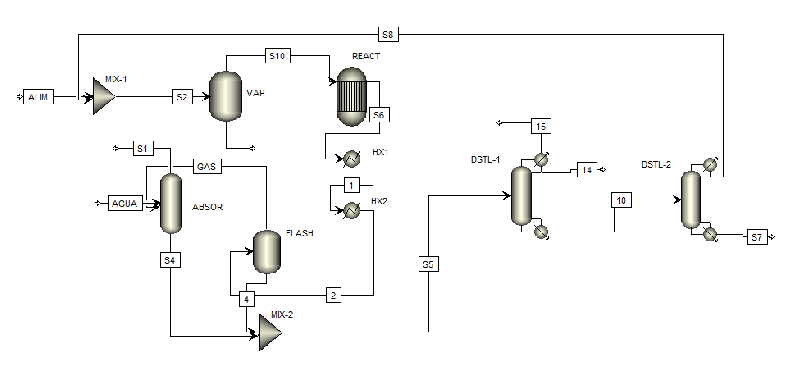
\includegraphics[width=16cm, height=8cm]{images/Diagramageneral.eps}
            \caption{Diagrama general del proceso simulado en Aspen Plus.}
            \label{fig:DiagramaCHIDO}
        \end{figure}

    \subsection*{Desarrollo del sistema de control}
    Para el sistema de control es necesario obtener la funciones transferencia a partir de las ecuaciones de balance de masa  del reactor además de los valores en estado estacionario  e iniciales.
    \paragraph{}
    Debido a que solo nos interesa la temperatura del flujo de entrada, nos centraremos en los balances para $A$, $T_r$ y $T_j$. Una vez que se tienen las ecuaciones se procede a linealizar las mismas.\\
    Se definen las variables de desviacion:\\
        $\Bar{C_A}= C_A - C_{As} $  ,  $\Bar{T}= T - T_s $  , $\Bar{T_j}= T_j - T_{js}$y $\Bar{F_j}= F_j - F_{js}$   


    \paragraph{}
    Los valores de nuestro sistema son:\\
        \begin{multicols}{2}
        %Para el calculos de las constantes
        \setlength{\parindent}{0cm}
        $F_{rs} = 0.0972\: m^3/s $\\ 
        $F_{j} = 0.01\: m^3/s$\\
        $k_0 = 3.51\: \times 10^5  1/s$ \\
        $UA = 1668431: J/s$\\
        $E = 72380\: J/mol\:K $\\
        $C_{pr} = 2500 \: J/Kg\:K$\\
        $C_{j} = 1700 \: J/Kg\:K$\\
        $ V_r = 3 \: m^3$\\
        $ V_j = 1 \: m^3$\\
        $ \Delta H_{rxn}= 70000 \:J/mol$\\
        $\rho_r = 785\:Kg/m^3$ \\
        $\rho_j = 970\:Kg/m^3$ \\
        $R = 8.314\: J/mol\: K$\\
        $T_s = 624\:K$\\
        $T_{j0} = 427\:K$\\
        $T_{j} = 327\:K$\\
        $C_{A0} = 526 \: mol/m^3$\\
        $C_{As} = 50.3168 \: mol/m^3$\\
        \end{multicols}

    Sustituyendo los valores en las ecuaciones \ref{balanceA}, \ref{energia} y \ref{energiachaqueta}, los balances quedan de la siguiente manera:\\

        $\dfrac{\partial (\ref{balanceA}) }{\partial C_A} = -\dfrac{F_r}{V_r}\Bar{C_A} = -0.0324\:\Bar{C_A}$

        $\dfrac{\partial (\ref{energia}) }{\partial C_A} = -\frac{\mathrm{\Delta H_{rxn}}\,\mathrm{k_0}\,{\mathrm{e}}^{-\frac{E}{R\,\mathrm{T_{rs}}}}}{\mathrm{C_{pr}}\,\mathrm{\rho_r}}\Bar{C_A}= - 0.0109 \:\Bar{C_A}$

        $\dfrac{\partial (\ref{energiachaqueta}) }{\partial C_A} = 0$

%% Para  Tr 

        $ \dfrac{\partial (\ref{balanceA}) }{\partial T_r} = -\frac{E\,\mathrm{k_0}\,{\mathrm{e}}^{-\frac{E}{R\,\mathrm{T_{rs}}}}}{R\,{\mathrm{T_{rs}}}^2}\Bar{T_r} = -0.0068 \:\Bar{T_r}$

        $ \dfrac{\partial (\ref{energia}) }{\partial T_r} = -\frac{F_r}{V_r}-\frac{\mathrm{UA}}{\mathrm{C_{pr}}\,V_r\,\mathrm{\rho_r}}-\frac{\mathrm{C_{As}}\,\mathrm{\Delta  H_{rxn}}\,E\,\mathrm{k_0}\,{\mathrm{e}}^{-\frac{E}{R\,\mathrm{T_{rs}}}}}{\mathrm{C{pr}}\,R\,{\mathrm{T_{rs}}}^2\,\mathrm{\rho_r}}\Bar{T_r}= -0.3281 \:\Bar{T_r}$

        $\dfrac{\partial (\ref{energiachaqueta}) }{\partial T_r} = \frac{\mathrm{UA}}{\mathrm{C_{pj}}\,\mathrm{V_j}\,\mathrm{\rho_j}}\Bar{T_r} = 1.0118  \:\Bar{T_r}$

%% Para  Tj

        $ \dfrac{\partial (\ref{balanceA}) }{\partial T_j} = 0$

        $ \dfrac{\partial (\ref{energia}) }{\partial T_j} =\frac{\mathrm{UA}}{\mathrm{C_{pr}}\,V_r\,\mathrm{\rho_r}} \Bar{T_j} = 0.2834 \:\Bar{T_j}$

        $ \dfrac{\partial (\ref{energiachaqueta}) }{\partial T_j} = -\frac{\mathrm{F_j}}{\mathrm{V_j}}-\frac{\mathrm{UA}}{\mathrm{C_{pj}}\,\mathrm{V_j}\,\mathrm{\rho_j}} \Bar{T_j} = -1.0218 \:\Bar{T_j}$

%% Para la  Vmanupulable
        $\dfrac{\partial (\ref{balanceA}) }{\partial F_j} = 0$

        $ \dfrac{\partial (\ref{energia}) }{\partial F_j} = 0$

        $ \dfrac{\partial (\ref{energiachaqueta}) }{\partial F_j} = -\frac{\mathrm{T_j}-\mathrm{T_j}_{0}}{\mathrm{V_j}}\Bar{F_j}= 88\Bar{F_j} $ \\
    En forma de matriz de  tiene:\\

        \begin{center}
            \begin{bmatrix}

            s + 0.0324 &   0.0068   &         0\\
            0.0109     & s + 0.3281 &   -0.2834\\
            0          &  - 1.0118  &  s+  1.0218\\ 
            \end{bmatrix}
            
            \begin{bmatrix}
            0\\
            0\\
            88
            \end{bmatrix}
        \end{center}
    \paragraph{}
    Realizando las transformadas de Laplace correspondiente se tiene que la funciones transferencia es:\\

        \begin{equation*}
            G(s) = \dfrac{88 s^2 + 31.72 s + 0.929}{s^{3} + 1.382\:s^2 + 0.09217\:s + 0.001495 }
        \end{equation*}
    Para proponer el controlador se va a utilizar el método de Cohen-Coon por ser un lazo abierto y además se agrega un escalón unitario para tener un delay, por lo tanto, para calcular los parámetros de los diferentes  controladores se utilizan las ecuaciones que se muestran en la \textit{Tabla \ref{tabla:ecucontrol}} . 

    %% Aqui se agregó una tabla 

    \begin{table}[H]
    \caption{ Ecuaciones para el calculo de los valores de distintos tipos de controladores por el método de Cohen-Coon} 
    \centering
    \begin{tabular}{llll}
    \hline
    Controlador & $K_c$ & $\tau_D$ & $\tau_I$  \\
    \hline
    P                   & $\frac{\tau}{K\:t_d}\left(1 +\frac{t_d}{3 \tau}  \right) $   & -   &-     \\
    PI                  & $\frac{\tau}{K\:t_d}\left(0.9 +\frac{t_d}{12 \tau}  \right) $   & $ t_d \frac{30 + 3(t_d/\tau)}{9+20(t_d/\tau)}$   &     \\
    PID                 &  $\frac{\tau}{K\:t_d}\left(4/3 +\frac{t_d}{4 \tau}  \right) $  & $ t_d \frac{32 + 6(t_d/\tau)}{13+8(t_d/\tau)}$   &  $ t_d \frac{4}{11+2(t_d/\tau)}$   \\
    \hline
    \end{tabular}
    \label{tabla:ecucontrol}
\end{table}


    donde $t_d$ es el delay,
    $K$ se calcula mediante: $B/S $ 
    donde $S$ es la pendiente a la tangente de la curva de reacciona lazo abierto y $B$ y el escalón en señal de control,$A$  es la magnitud del escalón. 

    \subsection*{Desarrollo de la viabilidad sustentable}
    En cuanto al objetivo de analizar el impacto económico, social y ambiental de la producción de acetona es necesario conocer las normas que regulan las concentraciones de acetona en distintos ambientes, descargas industriales en agua, suelo y aire. Así como los aspectos que alteren el entorno  social de los alrededores de la ubicación de la planta.
    El cumplimiento de los objetivos  para este proyecto es una serie de pasos para alcanzar la meta principal que es un análisis  de la producción de  acetona, tomando en cuenta que no solo este proceso afecta al sitio  donde se lleva a cabo la producción, si no que afecta  de diversas maneras a su entorno y a una parte de la sociedad

    \subsection*{Viabilidad sustentable económica}
    \subsubsection*{Importaciones y exportaciones de acetona}
    Las importaciones realizadas en los últimos 5 años vienen principalmente de Estados Unidos, Taiwán y Bélgica. En la \textit{Figura \ref{graf_acetona}} se muestran los respectivos porcentajes.

        \begin{figure}[H]
            \centering
            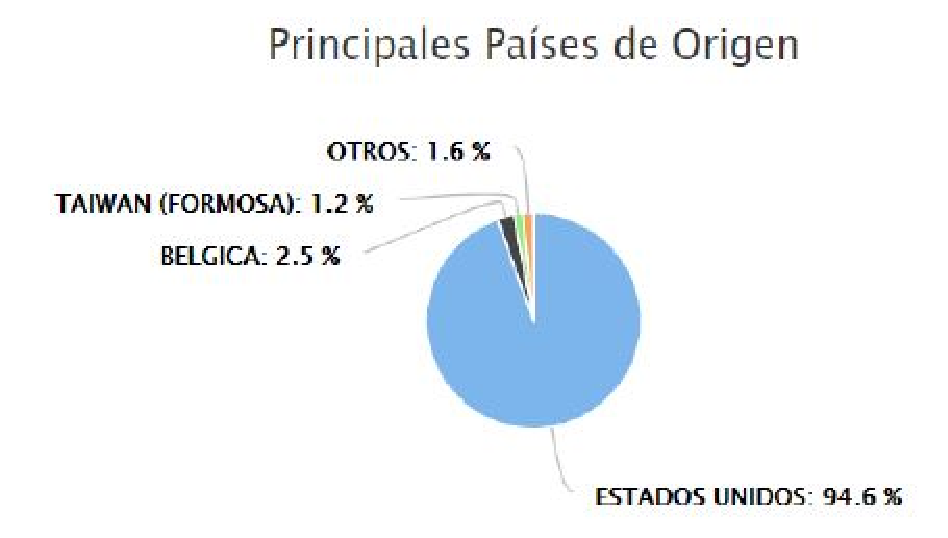
\includegraphics[scale= 0.7]{images/importacetona.eps}
            \caption{Origen importaciones acetona}
            \label{graf_acetona}
        \end{figure}

    Del 2015 al 2020 el valor de las importaciones a México asciende a \$ 351,868,389 USD y las exportaciones a \$ 13,166,844, cantidades que indican que las importaciones han sido mayores y esto indica que hay un amplio campo de aprovechamiento en la producción de acetona nacional para crecer en el mercado internacional.

    \subsubsection*{Capacidad de la planta}
    En México la producción de acetona cae en la categoría de producción de petroquímicos intermedios. El último dato que se encontró registrado por el INEGI de la capacidad instalada para producción de acetona fue en 2007 de 24,113 ton/año \cite{INEGI2009}
    %(INEGI, 2010).

    Con base al estudio de mercado y tomando en cuenta las tendencias de consumo se estima que la capacidad de la planta sería de 6,660.2 ton/año de acetona, cubriendo, un 18.5\% de la producción anual de acetona estimada en el 2020 según las tendencias de demanda y crecimiento de este producto.

    Se establece que el tiempo de operación anual es de 300 días al año y operando un proceso continuo de 24 horas al día, se alcanzará una producción de 22.2 toneladas al día, que será la capacidad nominal de los equipos que se utilizaran en la planta.

    La capacidad se establece basándose en plantas ya existentes productoras de acetona, tomando en cuenta que una sobreproducción nacional puede causar pérdidas económicas.
    \subsubsection*{Costos de los equipos}

    Para calcular la sustentabilidad económica del proyecto utilizamos el \textbf{análisis económico de Aspen} el cual nos calcula los costos de los equipos, servicios, instalación y operación del proyecto, estos se muestran en las Tablas \ref{tab:equipos}, \ref{tab:servicios}, \ref{tab:serviciosxaño}, \ref{tab:manodeobra} y \ref{tab:resultados} en la sección de resultados, cabe destacar que la acetona se vende aproximadamente en $2.00$ USD por kg.

    \subsection*{Viabilidad sustentable ambiental}

    \subsubsection*{Aguas residuales}

    La corriente que sale por el fondo de la segunda torre de destilación es la única que contiene ''agua residual'', sin embargo, gracias a la tecnología seleccionada y al elevado porcentaje de rendimiento donde se obtiene un producto de alta pureza, esta corriente tiene una fracción mol de 0.9961 agua, por lo tanto, con un adecuado sistema es posible recircularla a nuestro proceso.

    \subsubsection*{Residuos atmosféricos}

    Los principales contaminantes atmosféricos que se pueden producir en planta son:\\

    \textbf{Emisiones directas}\\

    Son producidas en el reactor donde se producen vapores orgánicos volátiles cetónicos o alcohólicos, estos pueden ser tratados en una columna de desorción de gases donde se recupere materia prima o producto principal emitiendo gases al ambiente con el límite máximo permisible.\\

    \textbf{Emisiones indirectas}\\

    Son las que produce la combustión de gas natural, es un combustible más limpio que los combustibles derivados de petróleo. Una solución es alimentar aire en exceso para evitar las combustiones incompletas que emiten compuestos nitrogenados, sulfúricos, etc.


    \subsection*{Viabilidad sustentable social}
    La acetona es un solvente esencial para la industria cosmética y del cuidado personal. Se espera que el rápido crecimiento de la industria del cuidado personal en los países en desarrollo impulse la demanda del mercado de acetona. Se prevé que la industria mundial del cuidado personal crezca con una tasa compuesta anual de casi el 5,78\% en los próximos años. Las economías emergentes, como los países de Asia-Pacífico y América Latina, tienen un enorme potencial de crecimiento para la industria del cuidado personal.


\section*{Resultados}
    Los parámetros de operación de las torres de destilación a partir de su simulación 
    en columnas DSTWU se muestran en las Tablas \ref{Parametros_DSTWU-1} y 
    \ref{Parametros_DSTWU-2}.

\begin{table}[H]
    \centering
    \caption{\textit{Parámetros de DSTWU-1}}
    \label{Parametros_DSTWU-1}
    \begin{tabular}{lll}
    \hline
    \multicolumn{2}{l}{DSTWU-1}                                           & Unidades \\
    \hline
    Relación mínima de reflujo                              & 1.9446      &          \\
    Relación de reflujo real                                & 2.7800      &          \\
    Número mínimo de etapas                                 & 18.2820     &          \\
    Número de etapas reales                                 & 31.8299     &          \\
    Etapa de alimentación                                   & 16.5290     &          \\
    Número de etapas reales por encima de la alimentación   & 15.5290     &          \\
    Requerimiento del hervidor                              & 129264.7000 & cal/s    \\
    Requerimiento del condensador                           & 112396.9630 & cal/s    \\
    Temperatura del destilado                               & 47.2418     & C        \\
    Temperatura inferior                                    & 81.3112     & C        \\
    Fracción para alimentación de destilado                 & 0.4468      &          \\ \hline
    \end{tabular}
\end{table}
\begin{table}[H]
    \centering
    \caption{\textit{Parámetros de DSTWU-2}}
    \label{Parametros_DSTWU-2}
    \begin{tabular}{lll}
    \hline
    \multicolumn{2}{l}{DSTWU-2}                      & Unidades    \\ \hline
    Relación mínima de reflujo         & 0.1209     &          \\
    Relación de reflujo real           & 0.8450     &          \\
    Número mínimo de etapas            & 1.7836     &          \\
    Número de etapas reales            & 2.9400     &          \\
    Etapa de alimentación              & 2.2000     &          \\
    Número de etapas reales por encima de la alimentación & 1.9448     &
    \\Requerimiento del hervidor    & 14712.0420 & cal/s \\
    Requerimiento del condensador         & 13522.2045 & cal/s  \\
    Temperatura del destilado          & 76.9745    & C        \\
    Temperatura inferior                & 94.9141    & C        \\
    Fracción para alimentación de destilado       & 0.1478     &   \\ \hline
    \end{tabular}
\end{table}

    Una vez realizada la simulación, se obtuvieron los valores que se muestran en las Tablas
    \ref{Tabla resultados}, \ref{cont_tab_3} y \ref{Continuacion resultados 2} para cada una
    de las corrientes y el gráfico que se muestra en la \textit{Figura \ref{fig:frac_mol}}. 
    Este gráfico nos muestra el número de etapas en la columna DSTL-1 y la fracción mol de acetona,
    agua, IPA e hidrógeno. La línea en color rosa nos representa la relación de fracción mol líquida 
    de acetona respecto al número de etapa, es por ello que en la etapa número uno se tiene una 
    fracción mol de aproximadamente 0.99 de acetona, ya que es por la parte superior de nuestra 
    columna por donde sale nuestra corriente de interés que es la acetona. Conforme avanza el
    número de etapas esta línea va hacia bajo hasta llegar a cero, esto se debe a que no hay
    pérdida de acetona en el fondo de nuestra columna. Por el contrario, la corriente que sale
    por el fondo y conecta a nuestra columna de destilación DSTL-2 es 0.946 fracción mol de 
    agua y 0.054 fracción mol de IPA. La segunda columna de destilación nos permite recuperar el
    IPA por la parte de arriba de nuestra columna la cual es recirculada al inicio de nuestro 
    proceso, mientras que en el fondo se obtiene una fracción mol de 0.996 de agua.

\begin{table}[H]
    \centering
    \caption{\textit{Tabla de resultados de las corrientes del proceso.}}
    \label{Tabla resultados}
    \begin{tabular}{lllllll}
    \hline
    \multicolumn{7}{l}{Reporte de corrientes}                                               \\
    \hline
    Descripción    & Unidades   & 1          & 2         & 4         & 10          & 14        \\
    \hline
    Proviene           &         & HX1        & HX2       & FLASH     & DSTL-1      & DSTL-1    \\
    Hacia             &         & HX2        & FLASH     & MIX-2     & DSTL-2      &           \\
    Fase          &         &            &           & Liquido    & Liquido      & Liquido    \\
    Temperatura    & K       & 318        & 293       & 293       & 356.2272693 & 320.39    \\
    Presión       & atm     & 1          & 1         & 1.5       & 1           & 1         \\
    Densidad    & gm/cc   & 0.0014     & 0.0025    & 0.8206    & 0.8955      & 0.7622    \\
    \textbf{Flujo molar}     & kmol/hr & 45.8038    & 45.8038   & 25.8715   & 19.7348     & 16.1244   \\
    WATER          & kmol/hr & 10.1073    & 10.1073   & 9.9230    & 18.6759     & 0.1593    \\
    IPA            & kmol/hr & 1.1010     & 1.1010    & 1.0597    & 1.0589      & 0.0376    \\
    ACETONE        & kmol/hr & 17.2977    & 17.2977   & 14.8835   & 0           & 15.9268   \\
    HYDROGEN       & kmol/hr & 17.2977    & 17.2977   & 0.0054    & 0           & 0.0007    \\
    \textbf{Frac mol} &         &            &           &           &             &           \\
    WATER          &         & 0.2207     & 0.2207    & 0.3836    & 0.9463      & 0.0099    \\
    IPA            &         & 0.0240     & 0.0240    & 0.0410    & 0.0537      & 0.0023    \\
    ACETONE        &         & 0.3776     & 0.3776    & 0.5753    & 0           & 0.9877    \\
    HYDROGEN       &         & 0.3776     & 0.3776    & 0.0002    & 0           & 0         \\
    \textbf{$\dot{m}$ másico}     & kg/hr   & 1287.7751  & 1287.7751 & 1106.8919 & 400.0852    & 930.1604  \\
    WATER          & kg/hr   & 182.0861   & 182.0861  & 178.7664  & 336.4521    & 2.8700    \\
    IPA            & kg/hr   & 66.1665    & 66.1665   & 63.6829   & 63.6330     & 2.2572    \\
    ACETONE        & kg/hr   & 1004.6523  & 1004.6523 & 864.4317  & 0.0001      & 925.0318  \\
    HYDROGEN       & kg/hr   & 34.8701    & 34.8701   & 0.0108    & 0           & 0.0013    \\
    \textbf{Frac masa} &         &            &           &           &             &           \\
    WATER          &         & 0.1414     & 0.1414    & 0.1615    & 0.8410      & 0.0031    \\
    IPA            &         & 0.0514     & 0.0514    & 0.0575    & 0.1590      & 0.0024    \\
    ACETONE        &         & 0.7801     & 0.7801    & 0.7810    & 0           & 0.9945    \\
    HYDROGEN       &         & 0.0271     & 0.0271    & 0         & 0           & 0         \\
    $\dot{Q}$   & l/min   & 15246.244 & 8637.2997 & 22.4819   & 7.4461      & 20.3397 \\  \hline
    \end{tabular}
\end{table}

\begin{table}[H]
    \centering
    \caption{\textit{Continuación Tabla 3}}\begin{tabular}{lllllll}
    \label{cont_tab_3}
    \hline
    Descripción    & 15     & AGUA     & ALIM      & GAS       & S1        & S2         \\ \hline
    Proviene            & DSTL-1 &          &           & FLASH     & ABSOR     & MIX-1      \\
     Hacia             &        & ABSOR    & MIX-1     & ABSOR     &           & VAP        \\
    Fase          & Vapor  & Liquido   & Liquido   & Vapor     & Vapor     & Liquid     \\
    Temperatura   & 320.39 & 320      & 320       & 293       & 318.7346  & 322.5447   \\
    Presión        & 1      & 1.5      & 1         & 1.5       & 1.5       & 0.9869     \\
    Densidad   & 0.0016 & 0.9726   & 0.7879    & 0.0006    & 0.0004    & 0.7874     \\
    \textbf{Flujo molar}     & 0.0223 & 10       & 25.9800   & 19.9322   & 19.9242   & 28.5061    \\
    WATER          & 0.0001 & 10       & 8.5734    & 0.1843    & 1.2731    & 10.1073    \\
    IPA            & 0      & 0        & 17.4066   & 0.0413    & 0.0047    & 18.3987    \\
    ACETONE        & 0.0161 & 0        & 0         & 2.4143    & 1.3555    & 1.36E-06   \\
    HYDROGEN       & 0.0060 & 0        & 0         & 17.2924   & 17.2910   & 0          \\
    \textbf{Frac mol} &        &          &           &           &           &            \\
    WATER          & 0.0055 & 1        & 0.3300    & 0.0092    & 0.0639    & 0.3546     \\
    IPA            & 0.0009 & 0        & 0.6700    & 0.0021    & 0.0002    & 0.6454     \\
    ACETONE        & 0.7219 & 0        & 0         & 0.1211    & 0.0680    & 4.79E-08   \\
    HYDROGEN       & 0.2717 & 0        & 0         & 0.8676    & 0.8678    & 0          \\
    $\dot{m}$ \textbf{ másico}     & 0.9492 & 180.1528 & 1200.5178 & 180.8833  & 136.7977  & 1287.7751  \\
    WATER          & 0.0022 & 180.1528 & 154.4522  & 3.3197    & 22.9345   & 182.0861   \\
    IPA            & 0.0012 & 0        & 1046.0656 & 2.4836    & 0.2805    & 1105.6889  \\
    ACETONE        & 0.9335 & 0        & 0         & 140.2206  & 78.7261   & 7.93E-05   \\
    HYDROGEN       & 0.0122 & 0        & 0         & 34.8593   & 34.8566   & 0          \\
    \textbf{Frac masa} &        &          &           &           &           &            \\
    WATER          & 0.0023 & 1        & 0.1287    & 0.0184    & 0.1677    & 0.1414     \\
    IPA            & 0.0013 & 0        & 0.8713    & 0.0137    & 0.0021    & 0.8586     \\
    ACETONE        & 0.9835 & 0        & 0         & 0.7752    & 0.5755    & 6.16E-08   \\
    HYDROGEN       & 0.0128 & 0        & 0         & 0.1927    & 0.2548    & 0          \\
    $\dot{Q}$   & 9.7558 & 3.0871   & 25.3945   & 5324.6572 & 5789.9982 & 27.2580   \\ \hline
    \end{tabular}
\end{table}

\begin{table}[H]
    \centering
    \caption{\textit{Continuación Tabla 3}}
    \label{Continuacion resultados 2}
    \begin{tabular}{llllll}
    \hline
    Descripción    & S4       & S5        & S7       & S8       & S10        \\ \hline
    Proviene             & ABSOR    & MIX-2     & DSTL-2   & DSTL-2   & VAP        \\
    Hacia              & MIX-2    & DSTL-1    &          & MIX-1    & REACT      \\
    Fase          & Liquido   &           & Liquido   & Liquido   & Vapor      \\
    Temperatura    & 303.7686 & 299.3965  & 369.6689 & 352.9200 & 389        \\
    Presión       & 1.5      & 1.5       & 0.9869   & 0.9869   & 2.6        \\
    Densidad    & 0.9178   & 0.8275    & 0.9185   & 0.7835   & 0.0037     \\
    \textbf{Flujo molar}     & 10.0080  & 35.8814   & 17.2087  & 2.5261   & 28.5061    \\
    WATER          & 8.9112   & 18.8354   & 17.1420  & 1.5339   & 10.1073    \\
    IPA            & 0.0367   & 1.0964    & 0.0667   & 0.9921   & 18.3987    \\
    ACETONE        & 1.0588   & 15.9429   & 1.16E-07 & 1.36E-06 & 1.36E-06   \\
    HYDROGEN       & 0.0014   & 0.0067    & 0        & 0        & 0          \\
    \textbf{Frac mol} &          &           &          &          &            \\
    WATER          & 0.8904   & 0.5249    & 0.9961   & 0.6072   & 0.3546     \\
    IPA            & 0.0037   & 0.0306    & 0.0039   & 0.3928   & 0.6454     \\
    ACETONE        & 0.1058   & 0.4443    & 6.76E-09 & 5.40E-07 & 4.79E-08   \\
    HYDROGEN       & 0.0001   & 0.0002    & 0        & 0        & 0          \\
    $\dot{m}$ \textbf{ másico}     & 224.2384 & 1331.1947 & 312.8279 & 87.2573  & 1287.7751  \\
    WATER          & 160.5380 & 339.3243  & 308.8182 & 27.6339  & 182.0861   \\
    IPA            & 2.2031   & 65.8914   & 4.0097   & 59.6232  & 1105.6889  \\
    ACETONE        & 61.4945  & 925.9654  & 6.75E-06 & 7.93E-05 & 7.93E-05   \\
    HYDROGEN       & 0.0027   & 0.0135    & 0        & 0        & 0          \\
    \textbf{Frac masa} &          &           &          &          &            \\
    WATER          & 0.7159   & 0.2549    & 0.9872   & 0.3167   & 0.1414     \\
    IPA            & 0.0098   & 0.0495    & 0.0128   & 0.6833   & 0.8586     \\
    ACETONE        & 0.2742   & 0.6956    & 2.16E-08 & 9.08E-07 & 6.16E-08   \\
    HYDROGEN       & 1.22E-05 & 1.02E-05  & 0        & 0        & 0          \\
    $\dot{Q}$     & 4.0721   & 26.8117   & 5.6762   & 1.8561   & 5832.7416 \\ \hline
    \end{tabular}
\end{table}
    

        \begin{figure}[H]
            \centering
            \includegraphics[scale=0.8]{images/etapas_vs_fracmol.PNG}
            \caption{Etapas vs Fracción mol de la acetona, agua, IPA e hidrógeno.}
            \label{fig:frac_mol}
        \end{figure}
    Para proponer nuestro sistema de control en el reactor mediante la relación de la 
    temperatura del reactor y la temperatura de la entrada de la chaqueta, se determinó 
    que la entrada manipulable  es la temperatura de la chaqueta $T_j$. En este caso como lo 
    indica el $\Delta H_{rxn} $ positivo, la reacción es endotérmica, por lo tanto es necesario
    calentar el reactor para llevarlo a la temperatura deseada. Con el balance de energía del 
    reactor se logró determinar la función de transferencia de nuestro proceso y mediante el 
    método de Cohen-Coon; ya que teníamos una función de transferencia a lazo abierto, se logró
    observar la estabilidad de nuestro reactor haciendo uso del software MATLAB como se muestra en 
    la Figura \ref{fig:unitario}.

\begin{table}[H]
    \caption{Valores para distintos tipos de controladores}
    \label{valore_controladores}
   \centering
   \begin{tabular}{llll}
   \hline
   Controlador & $K_c$ & $\tau_D$ & $\tau_I$  \\
   \hline
   P                   & 0.0064    & -   &-     \\
   PI                  &  0.0016  & 1.5023    & -    \\
   PID                 & 0.0048 & 7.5045   &0.0032   \\
   \hline
   \end{tabular}
\end{table}
   

        \begin{figure}[H]
            \centering
            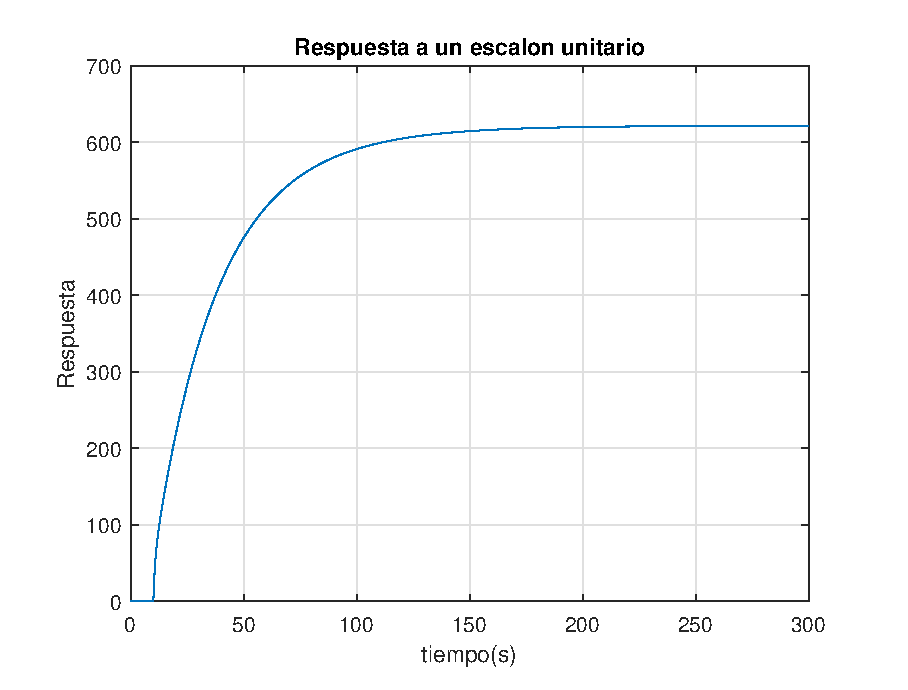
\includegraphics{images/unitarioM.eps}
            \caption{Respuesta del sistema ante un escalón unitario}
            \label{fig:unitario}
        \end{figure}

    \paragraph{}
    Para determinar la viabilidad económica del proyecto se tomó en cuenta el costo de los 
    equipos, su instalación, servicios, mano de obra operativa y de mantenimiento que nos 
    ofrece el análisis económico de Aspen que se muestra en las Tablas \ref{tab:equipos}, 
    \ref{tab:servicios}, \ref{tab:serviciosxaño}, \ref{tab:manodeobra} y \ref{tab:resultados}, 
    por nuestra parte determinamos el costo total de la materia prima y con base en el 
    análisis de mercado se determinaron las ventas totales del producto, una vez determinada 
    la tasa de retorno TIR se obtiene una tasa positiva lo cual indica que hemos tenido unos 
    beneficios mayores a la inversión realizada y por tanto hemos obtenido ganancias.
    \paragraph{}

\begin{table}[H]
    \centering
    \caption{Costo de equipos e instalación}
    \label{tab:equipos}
    \begin{tabular}{l|r|r}
    \hline
    \multicolumn{1}{c|}{Equipo} & \multicolumn{1}{c|}{Costo (USD)} & \multicolumn{1}{c}{Costo de instalación (USD)} \\ \hline
    Vaporizador                 & 15,600.00                        & 103,100.00                                     \\
    Reactor                     & 100,000.00                       & 250,000.00                                     \\
    Enfriador                   & 9,900.00                         & 99,600.00                                      \\
    Condensador                 & 10,000.00                           & 66,500.00                                      \\
    Separador flash             & 15,600.00                           & 96,000.00                                      \\
    Columna de absorción        & 41,300.00                           & 169,500                                        \\
    Columna de destilación 1    & 233,200.00                       & 652,600.00                                     \\
    Columna de destilación 2    & 56,900.00                           & 382,400.00                                     \\ \hline
    Total                       & 482,500.00                       & 1,819,700.00     \\ \hline                             
    \end{tabular}
\end{table}

\begin{table}[H]
    \centering
    \caption{Servicios}
    \label{tab:servicios}
    \hline 
    \resizebox{\textwidth}{!}{%
    \begin{tabular}{l|l|cc|c}
    \multicolumn{1}{c|}{Nombre} & \multicolumn{1}{c|}{Fluido} & Velocidad & Unidades de velocidad & Costo por hora (USD/H) \\ \hline
    Electricidad                &                             & 53.532    & KW                    & 4.14873                \\
    Agua de enfriamiento        & Agua                        & 0.019092  & MMGAL/H               & 2.29104                \\
    Refrigerante - Freon 12     & Refrigerante                & 8.414624  & KLB/H                 & 0.715243               \\
    Vapor 100PSI               & Vapor                       & 2.532263  & KLB/H                 & 20.612621 \\ \hline             
    \end{tabular}%
    }
\end{table}

\begin{table}[H]
    \centering
    \caption{Costo de servicios por año}
    \label{tab:serviciosxaño}
    
    \begin{tabular}{l|c}
    \hline 
      Servicio                    & \multicolumn{1}{l}{USD/año} \\ \hline
    Electricidad          & 36,367.8                      \\
    Servicios del proceso & 207,043                       \\ \hline
    Total                 & 243,411  \\ \hline                     
    \end{tabular}
\end{table}
    

    

\begin{table}[H]
    \centering
    \caption{Costo de mano de obra operativa y mantenimiento}
    \label{tab:manodeobra}
    \begin{tabular}{l|l|l}
    \hline 
    \textbf{Mano de obra}  &                    &            \\ \hline 
    Operadores por turno   &                    & 2          \\
    Costo unitario         & Costo/Operador/h   & 20         \\ \hline
    Total (USD)            & Costo/año          & 350,640.00 \\
                           &                    &            \\ \hline 
    \textbf{Mantenimiento} &                    &            \\ \hline 
    Costo/8000 h           &                    & 29100      \\ \hline 
    Total (USD)            & Costo/año          & 31,886.3   \\
                           &                    &            \\ \hline 
    \textbf{Supervisión}   &                    &            \\ \hline 
    Supervisores por turno &                    & 1          \\
    Costo unitario         & Costo/Supervisor/h & 35         \\ \hline
    Total (USD)                 & Costo/año          & 306,810   \\ \hline 
    \end{tabular}
\end{table}

\begin{table}[H]
    \centering
    \caption{Resumen de resultados del proyecto}
    \label{tab:resultados}
    \begin{tabular}{l|c} \hline 
    Costo de capital total del proyecto  [USD]                               & 5,673,990  \\
    Costo total de operación   [USD/año]                        & 1,557,120   \\
    Costo total de mano de obra operativa y mantenimiento [USD] & 689,336     \\
    Costo total de materia prima   [USD/año]                    & 708,644          \\
    Ventas totales de producto [USD/año]                        & 13,320,400
    
              \\
    Costo total de servicios   [USD/año]                        & 243,411     \\
    Costo de equipo [USD]                                       & 482,500     \\
    Costo total de instalación [USD]                            & 1,819,700 \\ \hline   
    \end{tabular}
\end{table}

    La tasa  de retorno TIR  a un periodo de 2 años es de:
    \textbf{2.104}

        $$0 = - 5,673,990 + \dfrac{13,320,400}{1+TIR} +\dfrac{13,320,400}{(1+TIR)^2}  $$
    Despejando para TIR se obtiene los 2.104 
\section*{Conclusiones}
El presente proyecto tuvo como base el proceso para producción de acetona descrito 
por %  es turton en el documento de luybel
Turton et al. Las condiciones de operación ahí planteadas para cada uno de los
equipos resultaron útiles para la simulación del mismo proceso a excepción de 
las columnas de destilación; estas tuvieron que ser primero simuladas como columna
DSTWU para una vez obtenidos los datos ser integradas en el proceso, además de 
realizar una modificación en la corriente de entrada del 50\% menos en la 
alimentación. Una vez llevada a cabo la simulación se logró obtener un producto con 
99\% de pureza, con esto  podemos decir que que nuestro primer objetivo estaba 
cumplido.
\paragraph{}
En cuanto al sistema de control se logro realizar una propuesta de control, 
mediante la relación de la temperatura del reactor y el flujo de entrada de  la 
chaqueta, por lo tanto la entrada manipulable es el flujo de entrada de la 
chaqueta $F_j$. En este caso como lo indica el $\Delta H_{rxn} $ positivo, la 
reacción es endotérmica, por lo tanto es necesario calentar el reactor para 
llevarlo a la temperatura deseada. Por esta razón el balance de energía del 
reactor es muy importante para controlar el proceso.
Para realizar los cálculos de los diferentes controladores (P,PI,PID) se logro 
realizar mediante el método de Cohen-Coon, el cual consideramos el mas sencillo 
para este caso, ya que teníamos la función de transferencia a lazo abierto.
 En este trabajo no se realizo un  análisis profundo sobre el  comportamiento 
 del sistema, es necesario un análisis posterior para tener una perspectiva más 
 completa de este proceso.
\paragraph{}
Respecto a la viabilidad sustentable de nuestro proyecto en el ámbito económico, 
ambiental y social consideramos que en general la producción de acetona a partir 
de alcohol isopropílico es una opción viable ya que representa un método amigable 
con el ambiente gracias a que los productos de desecho son mínimos y para la 
corriente que sale por el fondo de la segunda torre de destilación que es 
relativamente agua se podría proponer una torre de enfriamiento para 
recircularla al proceso. Con base al estudio de mercado, la producción 
de acetona es de importancia para producir otros productos de uso 
cotidiano, por lo tanto, el impacto social es positivo. Finalmente 
con los resultados obtenidos en el análisis económico; aunque la 
tasa de retorno resultó positiva, concluimos que sería posible optimizar 
nuestro proceso y así elevar la tasa de retorno.

%======================================%
%           Referencias                %
%======================================%


\bibliographystyle{apacite}
%\bibliographystyle{newapa}
\bibliography{referencias.bib}

\end{document}
